\scanpage{91}
et en composant (*) et (**) on trouve
\[
g_n(\underset{\sigma_{a_0}\rho}{\underline{\varepsilon_0}})
=g_n(\sigma_{a_0})g_n(\rho)
=\rho_1^{-1}\rho_\infty^{-1}
=(\rho_\infty\rho_1)^{-1}=\rho_0
\]
En résumé, on trouve donc
\[
\tag{98}
\left\{
\begin{gathered}
g_n:\Pi_1(X_n^*,D_n;P_{n+})\overset\sim\longrightarrow
\Pi_{0,3}/\langle\rho_1^2,\rho_\infty^n\rangle
=\Pi_1(\underset{\mathbb P^1_{\mathbb C}}{\underline{X_0}},
\underbrace{\infty\{0\}+2\{1\}+n\{\infty\}}_{\text{signature }\vec\nu_n};P_+)\\
\varepsilon_0\longmapsto\rho_0\\
\sigma_{a_0}\longmapsto\rho_1=\rho_1^{-1}\\
\rho\longmapsto\rho_\infty^{-1}
\end{gathered}
\right.
\]
Par le même principe, on trouve un isomorphisme
\[
\tag{99}
\begin{aligned}
g_n:\Pi_1(X_n^*,D_n\times\{1,\tau\};P_{n+})
&\overset\sim\longrightarrow\Pi_1(X_0,\underline{\vec\nu_n},\{1,\tau\};P_+)\\
\simeq\Pi_{\unsure{n|P}}^{D,\tau}\simeq\Pi_n^D.\{1,\widetilde\sigma_{a_0}\}
&\simeq(\Pi_{0,3}/\langle\rho_1^2,\rho_\infty^n\rangle).\{1,\widetilde\tau_\infty\}
\end{aligned}
\]

\margin{\uline{NB}
$\tau_\infty(\rho_0)=\rho_0^{-1}$\\
$\tau_\infty(\rho_1)=\rho_1^{-1}$\\
$\tau_\infty(\rho_\infty)=\rho_0(\rho_\infty^{-1})$\\
cf (80) dans le cas $n=3$, ici $\tau_\infty=\tau_{a_0}$ par définition \ldots}

qui prolonge $(97)=(98)$, et qui se calcule de la $\unsure{=|\overline m}$ façon. Il suffit, pour achever de déterminer $g_n$, de calculer sa valeur sur \deleted{$\unsure{\sigma_{a_0}}$}
$\widetilde\sigma_{a_0}=(1_{P_+},\widetilde\sigma^0_{a_0})$.
Ici $\widetilde\sigma^0_{a_0}$ agit sur $X_n$ par la symétrie par un grand cercle $P_\omega Q_{a_0}P_{\omega'}$, \deleted{\unsure{son}} son image dans
$\Pi_1(X_n^*,D_n\times\{1,\tau\};P)$ est défini par le chemin \deleted{$\unsure{P}$}
\[
P'=\widetilde\sigma^0_{a_0}(P)\longrightarrow P
\]
donné par $\alpha\circ\alpha'^{-1}$, où $\alpha'=\widetilde\sigma^0_{a_0}(\alpha)$, ce chemin est homotope dans $X_n^{\unsure{2|*}}$ au chemin $\widetilde\alpha_\sigma$, \deleted{qui} dans $X_n^{\unsure{***|**}}$, qui franchit la subdivision barycentrique une seule fois, en $P_+Q_{a_0}$ $(\overset{g_n}\longmapsto(\infty,1))$.

\figure{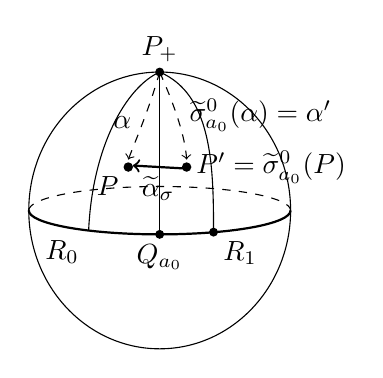
\begin{tikzpicture}[scale=.95]
\draw (0,0) ellipse (1.75 and 1.85);
\draw[thick] (-1.75,0) arc[start angle=180,end angle=360,x radius=1.75,y radius=.32];
\draw[dashed] (-1.75,0) arc[start angle=180,end angle=0,x radius=1.75,y radius=.32];
\draw (-.95,-.27) .. controls (-.9,.85) and (-.45,1.65) .. (0,1.85)
 .. controls (.7,1.55) and (.72,.6) .. (.72,-.29);
\draw (0,1.85) -- (0,-.32);
\fill (0,1.85) circle (1.7pt); \node[above] at (0,1.85) {$P_+$};
\node[below left] at (-.95,-.27) {$R_0$};
\fill (0,-.32) circle (1.7pt); \node[below] at (0,-.32) {$Q_{a_0}$};
\fill (.72,-.29) circle (1.7pt); \node[below right] at (.72,-.29) {$R_1$};
\fill (-.42,.58) circle (1.8pt); \node[below left] at (-.42,.58) {$P$};
\fill (.36,.58) circle (1.8pt); \node[right] at (.36,.58) {$P'=\widetilde\sigma^0_{a_0}(P)$};
\draw[dashed,->] (0,1.85) .. controls (-.14,1.36) and (-.3,.99) .. (-.42,.68);
\node[left] at (-.25,1.17) {$\alpha$};
\draw[dashed,->] (0,1.85) .. controls (.2,1.4) and (.34,.99) .. (.36,.68);
\node[right] at (.27,1.27) {$\widetilde\sigma^0_{a_0}(\alpha)=\alpha'$};
\draw[thick,->] (.35,.56) -- (-.36,.6);
\node[below] at (-.02,.58) {$\widetilde\alpha_\sigma$};
\end{tikzpicture}}

\margin{90}
